\documentclass[twoside]{book}

% Packages required by doxygen
\usepackage{fixltx2e}
\usepackage{calc}
\usepackage{doxygen}
\usepackage[export]{adjustbox} % also loads graphicx
\usepackage{graphicx}
\usepackage[utf8]{inputenc}
\usepackage{makeidx}
\usepackage{multicol}
\usepackage{multirow}
\PassOptionsToPackage{warn}{textcomp}
\usepackage{textcomp}
\usepackage[nointegrals]{wasysym}
\usepackage[table]{xcolor}

% Font selection
\usepackage[T1]{fontenc}
\usepackage[scaled=.90]{helvet}
\usepackage{courier}
\usepackage{amssymb}
\usepackage{sectsty}
\renewcommand{\familydefault}{\sfdefault}
\allsectionsfont{%
  \fontseries{bc}\selectfont%
  \color{darkgray}%
}
\renewcommand{\DoxyLabelFont}{%
  \fontseries{bc}\selectfont%
  \color{darkgray}%
}
\newcommand{\+}{\discretionary{\mbox{\scriptsize$\hookleftarrow$}}{}{}}

% Page & text layout
\usepackage{geometry}
\geometry{%
  a4paper,%
  top=2.5cm,%
  bottom=2.5cm,%
  left=2.5cm,%
  right=2.5cm%
}
\tolerance=750
\hfuzz=15pt
\hbadness=750
\setlength{\emergencystretch}{15pt}
\setlength{\parindent}{0cm}
\setlength{\parskip}{3ex plus 2ex minus 2ex}
\makeatletter
\renewcommand{\paragraph}{%
  \@startsection{paragraph}{4}{0ex}{-1.0ex}{1.0ex}{%
    \normalfont\normalsize\bfseries\SS@parafont%
  }%
}
\renewcommand{\subparagraph}{%
  \@startsection{subparagraph}{5}{0ex}{-1.0ex}{1.0ex}{%
    \normalfont\normalsize\bfseries\SS@subparafont%
  }%
}
\makeatother

% Headers & footers
\usepackage{fancyhdr}
\pagestyle{fancyplain}
\fancyhead[LE]{\fancyplain{}{\bfseries\thepage}}
\fancyhead[CE]{\fancyplain{}{}}
\fancyhead[RE]{\fancyplain{}{\bfseries\leftmark}}
\fancyhead[LO]{\fancyplain{}{\bfseries\rightmark}}
\fancyhead[CO]{\fancyplain{}{}}
\fancyhead[RO]{\fancyplain{}{\bfseries\thepage}}
\fancyfoot[LE]{\fancyplain{}{}}
\fancyfoot[CE]{\fancyplain{}{}}
\fancyfoot[RE]{\fancyplain{}{\bfseries\scriptsize Generated by Doxygen }}
\fancyfoot[LO]{\fancyplain{}{\bfseries\scriptsize Generated by Doxygen }}
\fancyfoot[CO]{\fancyplain{}{}}
\fancyfoot[RO]{\fancyplain{}{}}
\renewcommand{\footrulewidth}{0.4pt}
\renewcommand{\chaptermark}[1]{%
  \markboth{#1}{}%
}
\renewcommand{\sectionmark}[1]{%
  \markright{\thesection\ #1}%
}

% Indices & bibliography
\usepackage{natbib}
\usepackage[titles]{tocloft}
\setcounter{tocdepth}{3}
\setcounter{secnumdepth}{5}
\makeindex

% Hyperlinks (required, but should be loaded last)
\usepackage{ifpdf}
\ifpdf
  \usepackage[pdftex,pagebackref=true]{hyperref}
\else
  \usepackage[ps2pdf,pagebackref=true]{hyperref}
\fi
\hypersetup{%
  colorlinks=true,%
  linkcolor=blue,%
  citecolor=blue,%
  unicode%
}

% Custom commands
\newcommand{\clearemptydoublepage}{%
  \newpage{\pagestyle{empty}\cleardoublepage}%
}

\usepackage{caption}
\captionsetup{labelsep=space,justification=centering,font={bf},singlelinecheck=off,skip=4pt,position=top}

%===== C O N T E N T S =====

\begin{document}

% Titlepage & ToC
\hypersetup{pageanchor=false,
             bookmarksnumbered=true,
             pdfencoding=unicode
            }
\pagenumbering{alph}
\begin{titlepage}
\vspace*{7cm}
\begin{center}%
{\Large Middleware-\/soccer }\\
\vspace*{1cm}
{\large Generated by Doxygen 1.8.14}\\
\end{center}
\end{titlepage}
\clearemptydoublepage
\pagenumbering{roman}
\tableofcontents
\clearemptydoublepage
\pagenumbering{arabic}
\hypersetup{pageanchor=true}

%--- Begin generated contents ---
\chapter{Data Structure Index}
\section{Data Structures}
Here are the data structures with brief descriptions\+:\begin{DoxyCompactList}
\item\contentsline{section}{\mbox{\hyperlink{structevent}{event}} \\*Event from sensor }{\pageref{structevent}}{}
\item\contentsline{section}{\mbox{\hyperlink{structinterruption__event}{interruption\+\_\+event}} \\*Interruption event }{\pageref{structinterruption__event}}{}
\item\contentsline{section}{\mbox{\hyperlink{structoutput__envelope}{output\+\_\+envelope}} \\*Used to send messages to the output process }{\pageref{structoutput__envelope}}{}
\item\contentsline{section}{\mbox{\hyperlink{structposition}{position}} \\*Position coordinates in the game field }{\pageref{structposition}}{}
\item\contentsline{section}{\mbox{\hyperlink{structposition__event}{position\+\_\+event}} \\*Shows a game snapshot }{\pageref{structposition__event}}{}
\end{DoxyCompactList}

\chapter{File Index}
\section{File List}
Here is a list of all documented files with brief descriptions\+:\begin{DoxyCompactList}
\item\contentsline{section}{include/\mbox{\hyperlink{common_8h}{common.\+h}} \\*Common constants and definitions }{\pageref{common_8h}}{}
\item\contentsline{section}{include/\mbox{\hyperlink{output_8h}{output.\+h}} \\*Output.\+c function declaration }{\pageref{output_8h}}{}
\item\contentsline{section}{include/\mbox{\hyperlink{parser_8h}{parser.\+h}} \\*Parser.\+c function declaration }{\pageref{parser_8h}}{}
\item\contentsline{section}{include/\mbox{\hyperlink{possession_8h}{possession.\+h}} \\*Possession.\+c function declaration }{\pageref{possession_8h}}{}
\item\contentsline{section}{source/\mbox{\hyperlink{main_8c}{main.\+c}} \\*This file contains the main function which starts the program }{\pageref{main_8c}}{}
\item\contentsline{section}{source/\mbox{\hyperlink{output_8c}{output.\+c}} \\*This file defines a process, initialize by \mbox{\hyperlink{main_8c}{main.\+c}}, whose job is to compute and output the statistic of the game for each team and player }{\pageref{output_8c}}{}
\item\contentsline{section}{source/\mbox{\hyperlink{parser_8c}{parser.\+c}} \\*This file defines a process, initialized by \mbox{\hyperlink{main_8c}{main.\+c}}, whose job is to read game data }{\pageref{parser_8c}}{}
\item\contentsline{section}{source/\mbox{\hyperlink{possession_8c}{possession.\+c}} \\*This file defines a process, initialized by \mbox{\hyperlink{main_8c}{main.\+c}}, whose job is to establish which player, and thus team, has the ball, for each game positions update message from the \mbox{\hyperlink{parser_8h_a6b4f69b75cefd464a448d7dbf87576fa}{parser\+\_\+run}} process }{\pageref{possession_8c}}{}
\end{DoxyCompactList}

\chapter{Data Structure Documentation}
\hypertarget{structevent}{}\section{event Struct Reference}
\label{structevent}\index{event@{event}}


Event from sensor.  




{\ttfamily \#include $<$common.\+h$>$}



Collaboration diagram for event\+:\nopagebreak
\begin{figure}[H]
\begin{center}
\leavevmode
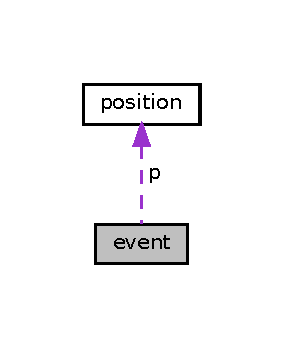
\includegraphics[width=136pt]{structevent__coll__graph}
\end{center}
\end{figure}
\subsection*{Data Fields}
\begin{DoxyCompactItemize}
\item 
\mbox{\Hypertarget{structevent_ad9b81c84e4a779b2a38b81e3918a9889}\label{structevent_ad9b81c84e4a779b2a38b81e3918a9889}} 
\mbox{\hyperlink{common_8h_af10e2dceeefdc0af7b5bab152a6380d2}{sid\+\_\+t}} {\bfseries sid}
\item 
\mbox{\Hypertarget{structevent_a88196c1fb2eb2b3764ff9d59926597b4}\label{structevent_a88196c1fb2eb2b3764ff9d59926597b4}} 
\mbox{\hyperlink{common_8h_aa141e5aeed9e5c126c44e1e0ca46a917}{picoseconds}} {\bfseries ts}
\item 
\mbox{\Hypertarget{structevent_a91726a3d7415e5d3933c1f900dfb56f4}\label{structevent_a91726a3d7415e5d3933c1f900dfb56f4}} 
\mbox{\hyperlink{structposition}{position}} {\bfseries p}
\end{DoxyCompactItemize}


\subsection{Detailed Description}
Event from sensor. 

Each event is characterized by\+:
\begin{DoxyItemize}
\item the id of the sensor which has generated it,
\item a timestamp,
\item the registered position. 
\end{DoxyItemize}

Definition at line 105 of file common.\+h.



The documentation for this struct was generated from the following file\+:\begin{DoxyCompactItemize}
\item 
include/\mbox{\hyperlink{common_8h}{common.\+h}}\end{DoxyCompactItemize}

\hypertarget{structinterruption__event}{}\section{interruption\+\_\+event Struct Reference}
\label{structinterruption__event}\index{interruption\+\_\+event@{interruption\+\_\+event}}


Interruption event.  




{\ttfamily \#include $<$common.\+h$>$}

\subsection*{Data Fields}
\begin{DoxyCompactItemize}
\item 
\mbox{\Hypertarget{structinterruption__event_a64b516cf84f0a790ca2fb38b751fce0f}\label{structinterruption__event_a64b516cf84f0a790ca2fb38b751fce0f}} 
\mbox{\hyperlink{common_8h_aa141e5aeed9e5c126c44e1e0ca46a917}{picoseconds}} {\bfseries start}
\item 
\mbox{\Hypertarget{structinterruption__event_abcb94fe0e71e1001d83ed2cfe80e8b50}\label{structinterruption__event_abcb94fe0e71e1001d83ed2cfe80e8b50}} 
\mbox{\hyperlink{common_8h_aa141e5aeed9e5c126c44e1e0ca46a917}{picoseconds}} {\bfseries end}
\end{DoxyCompactItemize}


\subsection{Detailed Description}
Interruption event. 

Each \mbox{\hyperlink{structinterruption__event}{interruption\+\_\+event}} is characterized by\+: the timestamps of beginning and end of the interruption. During an interruption event statistics are not updated. 

Definition at line 117 of file common.\+h.



The documentation for this struct was generated from the following file\+:\begin{DoxyCompactItemize}
\item 
include/\mbox{\hyperlink{common_8h}{common.\+h}}\end{DoxyCompactItemize}

\hypertarget{structoutput__envelope}{}\section{output\+\_\+envelope Struct Reference}
\label{structoutput__envelope}\index{output\+\_\+envelope@{output\+\_\+envelope}}


Used to send messages to the output process.  




{\ttfamily \#include $<$common.\+h$>$}

\subsection*{Data Fields}
\begin{DoxyCompactItemize}
\item 
\mbox{\Hypertarget{structoutput__envelope_a750e4b5fa22d3a61c559d648d024dba3}\label{structoutput__envelope_a750e4b5fa22d3a61c559d648d024dba3}} 
uint32\+\_\+t {\bfseries type}
\item 
\mbox{\Hypertarget{structoutput__envelope_a67cd433143ffcf2adb658b7f95860c11}\label{structoutput__envelope_a67cd433143ffcf2adb658b7f95860c11}} 
uint32\+\_\+t {\bfseries content}
\end{DoxyCompactItemize}


\subsection{Detailed Description}
Used to send messages to the output process. 

To avoid using multiple messages to know which M\+PI datatype the next message will be, we use a generic type that works for all the messages that we want to send, i.\+e. the print message from the parser and the result message from possession. Message types can be \mbox{\hyperlink{common_8h_a8da5798ca897bfce113cfdffeb72655f}{P\+O\+S\+I\+T\+I\+O\+N\+S\+\_\+\+M\+E\+S\+S\+A\+GE}}, \mbox{\hyperlink{common_8h_a091cde65311a49ac8f6680864db80171}{P\+R\+I\+N\+T\+\_\+\+M\+E\+S\+S\+A\+GE}}, \mbox{\hyperlink{common_8h_a04f4828ed043e0b47177dfa645656615}{P\+O\+S\+S\+E\+S\+S\+I\+O\+N\+\_\+\+M\+E\+S\+S\+A\+GE}} and \mbox{\hyperlink{common_8h_aa5e8a3ac8d01eeaaf829f70e2c26c5e0}{E\+N\+D\+O\+F\+G\+A\+M\+E\+\_\+\+M\+E\+S\+S\+A\+GE}}. 

Definition at line 145 of file common.\+h.



The documentation for this struct was generated from the following file\+:\begin{DoxyCompactItemize}
\item 
include/\mbox{\hyperlink{common_8h}{common.\+h}}\end{DoxyCompactItemize}

\hypertarget{structposition}{}\section{position Struct Reference}
\label{structposition}\index{position@{position}}


Position coordinates in the game field.  




{\ttfamily \#include $<$common.\+h$>$}

\subsection*{Data Fields}
\begin{DoxyCompactItemize}
\item 
\mbox{\Hypertarget{structposition_a0c61c6729b6e80082b774972c0cc2fba}\label{structposition_a0c61c6729b6e80082b774972c0cc2fba}} 
int32\+\_\+t {\bfseries x}
\item 
\mbox{\Hypertarget{structposition_a571440695a28e82fd4a074d7db3800a1}\label{structposition_a571440695a28e82fd4a074d7db3800a1}} 
int32\+\_\+t {\bfseries y}
\item 
\mbox{\Hypertarget{structposition_a2a609b23accc6ed1efca4fa86b569cf9}\label{structposition_a2a609b23accc6ed1efca4fa86b569cf9}} 
int32\+\_\+t {\bfseries z}
\end{DoxyCompactItemize}


\subsection{Detailed Description}
Position coordinates in the game field. 

x, y, z describe the position of the sensor in mm and the origin is the middle of a full size football field. 

Definition at line 91 of file common.\+h.



The documentation for this struct was generated from the following file\+:\begin{DoxyCompactItemize}
\item 
include/\mbox{\hyperlink{common_8h}{common.\+h}}\end{DoxyCompactItemize}

\hypertarget{structposition__event}{}\section{position\+\_\+event Struct Reference}
\label{structposition__event}\index{position\+\_\+event@{position\+\_\+event}}


Shows a game snapshot.  




{\ttfamily \#include $<$common.\+h$>$}



Collaboration diagram for position\+\_\+event\+:\nopagebreak
\begin{figure}[H]
\begin{center}
\leavevmode
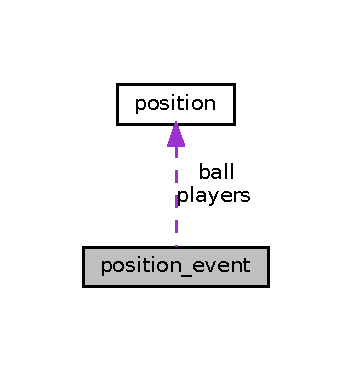
\includegraphics[width=169pt]{structposition__event__coll__graph}
\end{center}
\end{figure}
\subsection*{Data Fields}
\begin{DoxyCompactItemize}
\item 
\mbox{\Hypertarget{structposition__event_ae137a84e62d5845fd35ead6cd1514790}\label{structposition__event_ae137a84e62d5845fd35ead6cd1514790}} 
\mbox{\hyperlink{structposition}{position}} {\bfseries players} \mbox{[}17\mbox{]}
\item 
\mbox{\Hypertarget{structposition__event_a3296cf17f9475cc875f7927f6e24afa8}\label{structposition__event_a3296cf17f9475cc875f7927f6e24afa8}} 
\mbox{\hyperlink{structposition}{position}} {\bfseries ball}
\item 
\mbox{\Hypertarget{structposition__event_a42b0c3b25fb2f1298e6821d6744063c6}\label{structposition__event_a42b0c3b25fb2f1298e6821d6744063c6}} 
int32\+\_\+t {\bfseries interval\+\_\+id}
\end{DoxyCompactItemize}


\subsection{Detailed Description}
Shows a game snapshot. 

It is characterized by\+:
\begin{DoxyItemize}
\item an array with every player position,
\item the ball position,
\item the specific id of the interval in which the snapshot was taken. 
\end{DoxyItemize}

Definition at line 130 of file common.\+h.



The documentation for this struct was generated from the following file\+:\begin{DoxyCompactItemize}
\item 
include/\mbox{\hyperlink{common_8h}{common.\+h}}\end{DoxyCompactItemize}

\chapter{File Documentation}
\hypertarget{common_8h}{}\section{include/common.h File Reference}
\label{common_8h}\index{include/common.\+h@{include/common.\+h}}


Common constants and definitions.  


{\ttfamily \#include $<$stdint.\+h$>$}\newline
{\ttfamily \#include $<$mpi.\+h$>$}\newline
Include dependency graph for common.\+h\+:\nopagebreak
\begin{figure}[H]
\begin{center}
\leavevmode
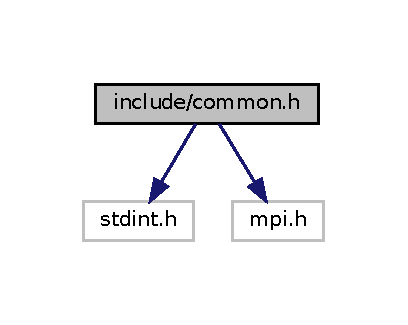
\includegraphics[width=196pt]{common_8h__incl}
\end{center}
\end{figure}
This graph shows which files directly or indirectly include this file\+:\nopagebreak
\begin{figure}[H]
\begin{center}
\leavevmode
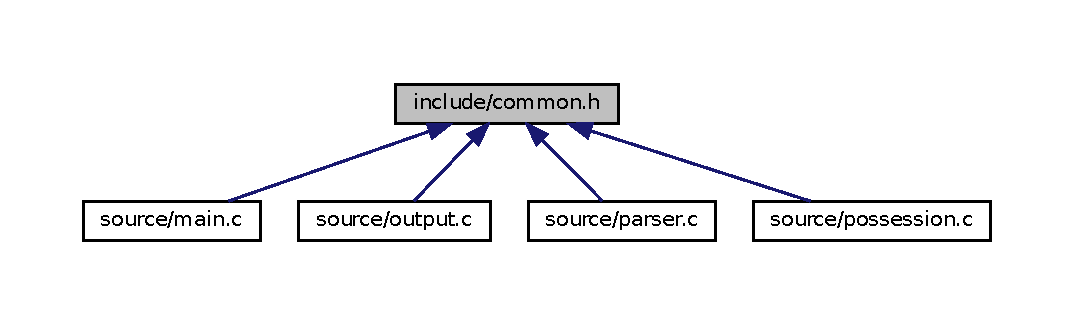
\includegraphics[width=350pt]{common_8h__dep__incl}
\end{center}
\end{figure}
\subsection*{Data Structures}
\begin{DoxyCompactItemize}
\item 
struct \mbox{\hyperlink{structposition}{position}}
\begin{DoxyCompactList}\small\item\em Position coordinates in the game field. \end{DoxyCompactList}\item 
struct \mbox{\hyperlink{structevent}{event}}
\begin{DoxyCompactList}\small\item\em Event from sensor. \end{DoxyCompactList}\item 
struct \mbox{\hyperlink{structinterruption__event}{interruption\+\_\+event}}
\begin{DoxyCompactList}\small\item\em Interruption event. \end{DoxyCompactList}\item 
struct \mbox{\hyperlink{structposition__event}{position\+\_\+event}}
\begin{DoxyCompactList}\small\item\em Shows a game snapshot. \end{DoxyCompactList}\item 
struct \mbox{\hyperlink{structoutput__envelope}{output\+\_\+envelope}}
\begin{DoxyCompactList}\small\item\em Used to send messages to the output process. \end{DoxyCompactList}\end{DoxyCompactItemize}
\subsection*{Macros}
\begin{DoxyCompactItemize}
\item 
\mbox{\Hypertarget{common_8h_a399dd27310d6f9c62ea851a7c0b6a7f0}\label{common_8h_a399dd27310d6f9c62ea851a7c0b6a7f0}} 
\#define \mbox{\hyperlink{common_8h_a399dd27310d6f9c62ea851a7c0b6a7f0}{P\+R\+G\+D\+E\+B\+UG}}~0
\begin{DoxyCompactList}\small\item\em Enables additional debug output. \end{DoxyCompactList}\item 
\mbox{\Hypertarget{common_8h_a32adf79142f0a426b5e782fb7cd4cad3}\label{common_8h_a32adf79142f0a426b5e782fb7cd4cad3}} 
\#define {\bfseries D\+BG}(x)~/$\ast$nothing$\ast$/
\item 
\mbox{\Hypertarget{common_8h_ac7dea2ffa0e506889c3d37c9aab67c6c}\label{common_8h_ac7dea2ffa0e506889c3d37c9aab67c6c}} 
\#define \mbox{\hyperlink{common_8h_ac7dea2ffa0e506889c3d37c9aab67c6c}{F\+U\+L\+L\+G\+A\+M\+E\+\_\+\+P\+A\+TH}}~\char`\"{}../datasets/full-\/game\char`\"{}
\begin{DoxyCompactList}\small\item\em Default path for the position events file. \end{DoxyCompactList}\item 
\mbox{\Hypertarget{common_8h_a705285bc2f2bdb3bd454ce8e8edf9057}\label{common_8h_a705285bc2f2bdb3bd454ce8e8edf9057}} 
\#define \mbox{\hyperlink{common_8h_a705285bc2f2bdb3bd454ce8e8edf9057}{S\+E\+C\+T\+O\+P\+IC}}~1000000000000
\begin{DoxyCompactList}\small\item\em Conversion factor from seconds to picosends. \end{DoxyCompactList}\item 
\mbox{\Hypertarget{common_8h_a5d1cf9a07c953e550f102d2152f33b0a}\label{common_8h_a5d1cf9a07c953e550f102d2152f33b0a}} 
\#define \mbox{\hyperlink{common_8h_a5d1cf9a07c953e550f102d2152f33b0a}{P\+O\+S\+S\+E\+S\+S\+I\+O\+N\+\_\+\+B\+U\+F\+F\+E\+R\+\_\+\+S\+I\+ZE}}~1
\begin{DoxyCompactList}\small\item\em Dimension of the results buffer to increase pipelining. \end{DoxyCompactList}\item 
\mbox{\Hypertarget{common_8h_a2fbe87a531354f51f8e3ea5815e82745}\label{common_8h_a2fbe87a531354f51f8e3ea5815e82745}} 
\#define \mbox{\hyperlink{common_8h_a2fbe87a531354f51f8e3ea5815e82745}{I\+G\+N\+O\+R\+E\+\_\+\+G\+O\+A\+L\+K\+E\+E\+P\+ER}}~0
\begin{DoxyCompactList}\small\item\em Set to 1 to remove the goalkeepers from the statistics. \end{DoxyCompactList}\end{DoxyCompactItemize}
\textbf{ }\par
\begin{DoxyCompactItemize}
\item 
\mbox{\Hypertarget{common_8h_a296fcf8956da16b4d0bf37dd7bfacc8b}\label{common_8h_a296fcf8956da16b4d0bf37dd7bfacc8b}} 
\#define \mbox{\hyperlink{common_8h_a296fcf8956da16b4d0bf37dd7bfacc8b}{F\+I\+R\+S\+T\+\_\+\+I\+N\+T\+E\+R\+R\+U\+P\+T\+I\+O\+NS}}~\char`\"{}../datasets/referee-\/events/Game Interruption/1st Half.\+csv\char`\"{}
\begin{DoxyCompactList}\small\item\em Default path for the game interruptions file. \end{DoxyCompactList}\item 
\mbox{\Hypertarget{common_8h_a99fae0dc2cdd4564a69701fb63ef71f1}\label{common_8h_a99fae0dc2cdd4564a69701fb63ef71f1}} 
\#define \mbox{\hyperlink{common_8h_a99fae0dc2cdd4564a69701fb63ef71f1}{S\+E\+C\+O\+N\+D\+\_\+\+I\+N\+T\+E\+R\+R\+U\+P\+T\+I\+O\+NS}}~\char`\"{}../datasets/referee-\/events/Game Interruption/2nd Half.\+csv\char`\"{}
\begin{DoxyCompactList}\small\item\em Default path for the game interruptions file. \end{DoxyCompactList}\end{DoxyCompactItemize}

\textbf{ }\par
\begin{DoxyCompactItemize}
\item 
\mbox{\Hypertarget{common_8h_a6aee779504f876f9bed834f36b392da9}\label{common_8h_a6aee779504f876f9bed834f36b392da9}} 
\#define \mbox{\hyperlink{common_8h_a6aee779504f876f9bed834f36b392da9}{X\+M\+IN}}~0
\begin{DoxyCompactList}\small\item\em Field dimensions. \end{DoxyCompactList}\item 
\mbox{\Hypertarget{common_8h_a0312cb6d6cbc719075d4e5380c387ab3}\label{common_8h_a0312cb6d6cbc719075d4e5380c387ab3}} 
\#define \mbox{\hyperlink{common_8h_a0312cb6d6cbc719075d4e5380c387ab3}{X\+M\+AX}}~52483
\begin{DoxyCompactList}\small\item\em Field dimensions. \end{DoxyCompactList}\item 
\mbox{\Hypertarget{common_8h_aa025181dff552575490c5148a493ff65}\label{common_8h_aa025181dff552575490c5148a493ff65}} 
\#define \mbox{\hyperlink{common_8h_aa025181dff552575490c5148a493ff65}{Y\+M\+IN}}~(-\/33960)
\begin{DoxyCompactList}\small\item\em Field dimensions. \end{DoxyCompactList}\item 
\mbox{\Hypertarget{common_8h_a610d6ad95b18966b70b6845de2a9c56b}\label{common_8h_a610d6ad95b18966b70b6845de2a9c56b}} 
\#define \mbox{\hyperlink{common_8h_a610d6ad95b18966b70b6845de2a9c56b}{Y\+M\+AX}}~33965
\begin{DoxyCompactList}\small\item\em Field dimensions. \end{DoxyCompactList}\end{DoxyCompactItemize}

\textbf{ }\par
\begin{DoxyCompactItemize}
\item 
\mbox{\Hypertarget{common_8h_a08ada8e459d6a78ab832b804fe67f9a1}\label{common_8h_a08ada8e459d6a78ab832b804fe67f9a1}} 
\#define \mbox{\hyperlink{common_8h_a08ada8e459d6a78ab832b804fe67f9a1}{G\+A\+M\+E\+\_\+\+S\+T\+A\+RT}}~10753295594424116
\begin{DoxyCompactList}\small\item\em Beginnings and ends of each half of the game. \end{DoxyCompactList}\item 
\mbox{\Hypertarget{common_8h_a00be8e922ee8c3e14442893f3dae22e5}\label{common_8h_a00be8e922ee8c3e14442893f3dae22e5}} 
\#define \mbox{\hyperlink{common_8h_a00be8e922ee8c3e14442893f3dae22e5}{F\+I\+R\+S\+T\+\_\+\+E\+ND}}~12557295594424116
\begin{DoxyCompactList}\small\item\em Beginnings and ends of each half of the game. \end{DoxyCompactList}\item 
\mbox{\Hypertarget{common_8h_ac73ff91e5f59bf1aeff42ba4f522725a}\label{common_8h_ac73ff91e5f59bf1aeff42ba4f522725a}} 
\#define \mbox{\hyperlink{common_8h_ac73ff91e5f59bf1aeff42ba4f522725a}{S\+E\+C\+O\+N\+D\+\_\+\+S\+T\+A\+RT}}~13086639146403495
\begin{DoxyCompactList}\small\item\em Beginnings and ends of each half of the game. \end{DoxyCompactList}\item 
\mbox{\Hypertarget{common_8h_a27f2d53d534caee2fd2b6252ef98abf8}\label{common_8h_a27f2d53d534caee2fd2b6252ef98abf8}} 
\#define \mbox{\hyperlink{common_8h_a27f2d53d534caee2fd2b6252ef98abf8}{G\+A\+M\+E\+\_\+\+E\+ND}}~14879639146403495
\begin{DoxyCompactList}\small\item\em Beginnings and ends of each half of the game. \end{DoxyCompactList}\end{DoxyCompactItemize}

\textbf{ }\par
\begin{DoxyCompactItemize}
\item 
\mbox{\Hypertarget{common_8h_a7a4a826a4a196d697aeb6257969fe233}\label{common_8h_a7a4a826a4a196d697aeb6257969fe233}} 
\#define \mbox{\hyperlink{common_8h_a7a4a826a4a196d697aeb6257969fe233}{P\+A\+R\+S\+E\+R\+\_\+\+R\+A\+NK}}~0
\begin{DoxyCompactList}\small\item\em Process identifiers. \end{DoxyCompactList}\item 
\mbox{\Hypertarget{common_8h_a3c6391770df18e1b2b4da8b2408fab24}\label{common_8h_a3c6391770df18e1b2b4da8b2408fab24}} 
\#define \mbox{\hyperlink{common_8h_a3c6391770df18e1b2b4da8b2408fab24}{O\+U\+T\+P\+U\+T\+\_\+\+R\+A\+NK}}~1
\begin{DoxyCompactList}\small\item\em Process identifiers. \end{DoxyCompactList}\item 
\mbox{\Hypertarget{common_8h_a938d3ae0f97952c11c7eacce1d463f39}\label{common_8h_a938d3ae0f97952c11c7eacce1d463f39}} 
\#define \mbox{\hyperlink{common_8h_a938d3ae0f97952c11c7eacce1d463f39}{P\+O\+S\+S\+E\+S\+S\+I\+O\+N\+\_\+\+R\+A\+NK}}~2
\begin{DoxyCompactList}\small\item\em Process identifiers. \end{DoxyCompactList}\end{DoxyCompactItemize}

\textbf{ }\par
\begin{DoxyCompactItemize}
\item 
\mbox{\Hypertarget{common_8h_a8da5798ca897bfce113cfdffeb72655f}\label{common_8h_a8da5798ca897bfce113cfdffeb72655f}} 
\#define \mbox{\hyperlink{common_8h_a8da5798ca897bfce113cfdffeb72655f}{P\+O\+S\+I\+T\+I\+O\+N\+S\+\_\+\+M\+E\+S\+S\+A\+GE}}~0
\begin{DoxyCompactList}\small\item\em Message type identifiers, defined as integers for use with M\+PI. \end{DoxyCompactList}\item 
\mbox{\Hypertarget{common_8h_a091cde65311a49ac8f6680864db80171}\label{common_8h_a091cde65311a49ac8f6680864db80171}} 
\#define \mbox{\hyperlink{common_8h_a091cde65311a49ac8f6680864db80171}{P\+R\+I\+N\+T\+\_\+\+M\+E\+S\+S\+A\+GE}}~1
\begin{DoxyCompactList}\small\item\em Message type identifiers, defined as integers for use with M\+PI. \end{DoxyCompactList}\item 
\mbox{\Hypertarget{common_8h_a04f4828ed043e0b47177dfa645656615}\label{common_8h_a04f4828ed043e0b47177dfa645656615}} 
\#define \mbox{\hyperlink{common_8h_a04f4828ed043e0b47177dfa645656615}{P\+O\+S\+S\+E\+S\+S\+I\+O\+N\+\_\+\+M\+E\+S\+S\+A\+GE}}~2
\begin{DoxyCompactList}\small\item\em Message type identifiers, defined as integers for use with M\+PI. \end{DoxyCompactList}\item 
\mbox{\Hypertarget{common_8h_aa5e8a3ac8d01eeaaf829f70e2c26c5e0}\label{common_8h_aa5e8a3ac8d01eeaaf829f70e2c26c5e0}} 
\#define \mbox{\hyperlink{common_8h_aa5e8a3ac8d01eeaaf829f70e2c26c5e0}{E\+N\+D\+O\+F\+G\+A\+M\+E\+\_\+\+M\+E\+S\+S\+A\+GE}}~3
\begin{DoxyCompactList}\small\item\em Message type identifiers, defined as integers for use with M\+PI. \end{DoxyCompactList}\end{DoxyCompactItemize}

\subsection*{Typedefs}
\begin{DoxyCompactItemize}
\item 
\mbox{\Hypertarget{common_8h_af10e2dceeefdc0af7b5bab152a6380d2}\label{common_8h_af10e2dceeefdc0af7b5bab152a6380d2}} 
typedef uint32\+\_\+t \mbox{\hyperlink{common_8h_af10e2dceeefdc0af7b5bab152a6380d2}{sid\+\_\+t}}
\begin{DoxyCompactList}\small\item\em Sensor id type. \end{DoxyCompactList}\item 
\mbox{\Hypertarget{common_8h_a7236ef194cc4c2220b9f7dc5e4777f22}\label{common_8h_a7236ef194cc4c2220b9f7dc5e4777f22}} 
typedef uint32\+\_\+t \mbox{\hyperlink{common_8h_a7236ef194cc4c2220b9f7dc5e4777f22}{player\+\_\+t}}
\begin{DoxyCompactList}\small\item\em Player type. \end{DoxyCompactList}\item 
\mbox{\Hypertarget{common_8h_aa141e5aeed9e5c126c44e1e0ca46a917}\label{common_8h_aa141e5aeed9e5c126c44e1e0ca46a917}} 
typedef uint64\+\_\+t \mbox{\hyperlink{common_8h_aa141e5aeed9e5c126c44e1e0ca46a917}{picoseconds}}
\begin{DoxyCompactList}\small\item\em Picoseconds type. \end{DoxyCompactList}\item 
typedef struct \mbox{\hyperlink{structposition}{position}} \mbox{\hyperlink{common_8h_a27f891824b3867d5b8b0be7426002623}{position}}
\begin{DoxyCompactList}\small\item\em Position coordinates in the game field. \end{DoxyCompactList}\item 
typedef struct \mbox{\hyperlink{structevent}{event}} \mbox{\hyperlink{common_8h_aed6db9834a774a2a7322cbe3e889a663}{event}}
\begin{DoxyCompactList}\small\item\em Event from sensor. \end{DoxyCompactList}\item 
typedef struct \mbox{\hyperlink{structinterruption__event}{interruption\+\_\+event}} \mbox{\hyperlink{common_8h_ad6587a779617aa61dba1bc2fed881298}{interruption\+\_\+event}}
\begin{DoxyCompactList}\small\item\em Interruption event. \end{DoxyCompactList}\item 
typedef struct \mbox{\hyperlink{structposition__event}{position\+\_\+event}} \mbox{\hyperlink{common_8h_adca5bead1943655023d990c0a2aea7df}{position\+\_\+event}}
\begin{DoxyCompactList}\small\item\em Shows a game snapshot. \end{DoxyCompactList}\end{DoxyCompactItemize}
\subsection*{Enumerations}
\begin{DoxyCompactItemize}
\item 
\mbox{\Hypertarget{common_8h_a089f166159fb19f10d81c65c1d8793a2}\label{common_8h_a089f166159fb19f10d81c65c1d8793a2}} 
enum \mbox{\hyperlink{common_8h_a089f166159fb19f10d81c65c1d8793a2}{sensor\+\_\+type\+\_\+t}} \{ {\bfseries P\+L\+A\+Y\+ER}, 
{\bfseries R\+E\+F\+E\+R\+EE}, 
{\bfseries B\+A\+LL}, 
{\bfseries N\+O\+NE}
 \}
\begin{DoxyCompactList}\small\item\em Each sensor registers data from a specific P\+L\+A\+Y\+ER, from the R\+E\+F\+E\+R\+EE or from the B\+A\+LL; N\+O\+NE as default case. \end{DoxyCompactList}\end{DoxyCompactItemize}


\subsection{Detailed Description}
Common constants and definitions. 

This file contains type definitions and global constants used by all processes. 

\subsection{Typedef Documentation}
\mbox{\Hypertarget{common_8h_aed6db9834a774a2a7322cbe3e889a663}\label{common_8h_aed6db9834a774a2a7322cbe3e889a663}} 
\index{common.\+h@{common.\+h}!event@{event}}
\index{event@{event}!common.\+h@{common.\+h}}
\subsubsection{\texorpdfstring{event}{event}}
{\footnotesize\ttfamily typedef struct \mbox{\hyperlink{structevent}{event}}  \mbox{\hyperlink{structevent}{event}}}



Event from sensor. 

Each event is characterized by\+:
\begin{DoxyItemize}
\item the id of the sensor which has generated it,
\item a timestamp,
\item the registered position. 
\end{DoxyItemize}\mbox{\Hypertarget{common_8h_ad6587a779617aa61dba1bc2fed881298}\label{common_8h_ad6587a779617aa61dba1bc2fed881298}} 
\index{common.\+h@{common.\+h}!interruption\+\_\+event@{interruption\+\_\+event}}
\index{interruption\+\_\+event@{interruption\+\_\+event}!common.\+h@{common.\+h}}
\subsubsection{\texorpdfstring{interruption\+\_\+event}{interruption\_event}}
{\footnotesize\ttfamily typedef struct \mbox{\hyperlink{structinterruption__event}{interruption\+\_\+event}}  \mbox{\hyperlink{structinterruption__event}{interruption\+\_\+event}}}



Interruption event. 

Each \mbox{\hyperlink{structinterruption__event}{interruption\+\_\+event}} is characterized by\+: the timestamps of beginning and end of the interruption. During an interruption event statistics are not updated. \mbox{\Hypertarget{common_8h_a27f891824b3867d5b8b0be7426002623}\label{common_8h_a27f891824b3867d5b8b0be7426002623}} 
\index{common.\+h@{common.\+h}!position@{position}}
\index{position@{position}!common.\+h@{common.\+h}}
\subsubsection{\texorpdfstring{position}{position}}
{\footnotesize\ttfamily typedef struct \mbox{\hyperlink{structposition}{position}}  \mbox{\hyperlink{structposition}{position}}}



Position coordinates in the game field. 

x, y, z describe the position of the sensor in mm and the origin is the middle of a full size football field. \mbox{\Hypertarget{common_8h_adca5bead1943655023d990c0a2aea7df}\label{common_8h_adca5bead1943655023d990c0a2aea7df}} 
\index{common.\+h@{common.\+h}!position\+\_\+event@{position\+\_\+event}}
\index{position\+\_\+event@{position\+\_\+event}!common.\+h@{common.\+h}}
\subsubsection{\texorpdfstring{position\+\_\+event}{position\_event}}
{\footnotesize\ttfamily typedef struct \mbox{\hyperlink{structposition__event}{position\+\_\+event}}  \mbox{\hyperlink{structposition__event}{position\+\_\+event}}}



Shows a game snapshot. 

It is characterized by\+:
\begin{DoxyItemize}
\item an array with every player position,
\item the ball position,
\item the specific id of the interval in which the snapshot was taken. 
\end{DoxyItemize}
\hypertarget{output_8h}{}\section{include/output.h File Reference}
\label{output_8h}\index{include/output.\+h@{include/output.\+h}}


\mbox{\hyperlink{output_8c}{output.\+c}} function declaration.  


This graph shows which files directly or indirectly include this file\+:\nopagebreak
\begin{figure}[H]
\begin{center}
\leavevmode
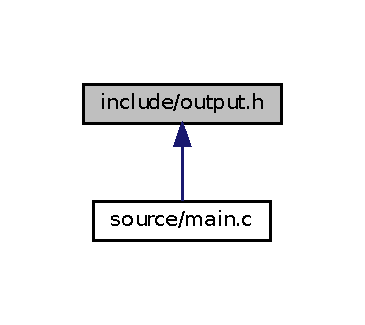
\includegraphics[width=175pt]{output_8h__dep__incl}
\end{center}
\end{figure}
\subsection*{Functions}
\begin{DoxyCompactItemize}
\item 
void \mbox{\hyperlink{output_8h_ac43f98545e1da1dbf0dff2d81ec06aef}{output\+\_\+run}} (M\+P\+I\+\_\+\+Datatype mpi\+\_\+output\+\_\+envelope, \mbox{\hyperlink{common_8h_aa141e5aeed9e5c126c44e1e0ca46a917}{picoseconds}} T)
\begin{DoxyCompactList}\small\item\em Starts the output process. \end{DoxyCompactList}\end{DoxyCompactItemize}


\subsection{Detailed Description}
\mbox{\hyperlink{output_8c}{output.\+c}} function declaration. 



\subsection{Function Documentation}
\mbox{\Hypertarget{output_8h_ac43f98545e1da1dbf0dff2d81ec06aef}\label{output_8h_ac43f98545e1da1dbf0dff2d81ec06aef}} 
\index{output.\+h@{output.\+h}!output\+\_\+run@{output\+\_\+run}}
\index{output\+\_\+run@{output\+\_\+run}!output.\+h@{output.\+h}}
\subsubsection{\texorpdfstring{output\+\_\+run()}{output\_run()}}
{\footnotesize\ttfamily void output\+\_\+run (\begin{DoxyParamCaption}\item[{M\+P\+I\+\_\+\+Datatype}]{mpi\+\_\+output\+\_\+envelope,  }\item[{\mbox{\hyperlink{common_8h_aa141e5aeed9e5c126c44e1e0ca46a917}{picoseconds}}}]{T }\end{DoxyParamCaption})}



Starts the output process. 

It keeps waiting for a P\+R\+I\+N\+T\+\_\+\+M\+E\+S\+S\+A\+GE or a P\+O\+S\+S\+E\+S\+S\+I\+O\+N\+\_\+\+M\+E\+S\+S\+A\+GE, from possession processes, until it receives the E\+N\+D\+\_\+\+O\+F\+\_\+\+G\+A\+ME message. After receiving a P\+O\+S\+S\+E\+S\+S\+I\+O\+N\+\_\+\+M\+E\+S\+S\+A\+GE, statistics are updated; after receiving a P\+R\+I\+N\+T\+\_\+\+M\+E\+S\+S\+A\+GE, interval and cumulative statistics are printed, and interval ones are reset; after receiving the E\+N\+D\+\_\+\+O\+F\+\_\+\+G\+A\+ME message, the process exits, after waiting for any pending request. If the received message is of any other type, the process abort.


\begin{DoxyParams}{Parameters}
{\em mpi\+\_\+output\+\_\+envelope} & M\+PI datatype of the received messages. \\
\hline
{\em T} & Length of time between outputs \\
\hline
\end{DoxyParams}


Definition at line 203 of file output.\+c.


\hypertarget{parser_8h}{}\section{include/parser.h File Reference}
\label{parser_8h}\index{include/parser.\+h@{include/parser.\+h}}


\mbox{\hyperlink{parser_8c}{parser.\+c}} function declaration.  


This graph shows which files directly or indirectly include this file\+:\nopagebreak
\begin{figure}[H]
\begin{center}
\leavevmode
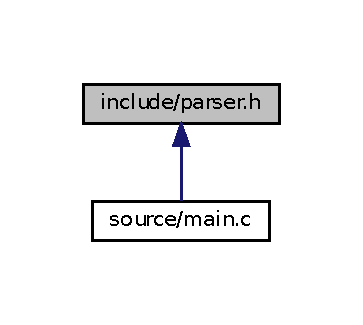
\includegraphics[width=174pt]{parser_8h__dep__incl}
\end{center}
\end{figure}
\subsection*{Functions}
\begin{DoxyCompactItemize}
\item 
void \mbox{\hyperlink{parser_8h_a6b4f69b75cefd464a448d7dbf87576fa}{parser\+\_\+run}} (M\+P\+I\+\_\+\+Datatype mpi\+\_\+position\+\_\+for\+\_\+possession\+\_\+type, M\+P\+I\+\_\+\+Datatype mpi\+\_\+output\+\_\+envelope, int possession\+\_\+processes, \mbox{\hyperlink{common_8h_aa141e5aeed9e5c126c44e1e0ca46a917}{picoseconds}} T, char $\ast$fullgame\+\_\+path, char $\ast$interr\+\_\+path\+\_\+one, char $\ast$interr\+\_\+path\+\_\+two)
\begin{DoxyCompactList}\small\item\em Starts the parser, which receives events from all sensors and communicates with the output and possession processes. \end{DoxyCompactList}\end{DoxyCompactItemize}


\subsection{Detailed Description}
\mbox{\hyperlink{parser_8c}{parser.\+c}} function declaration. 



\subsection{Function Documentation}
\mbox{\Hypertarget{parser_8h_a6b4f69b75cefd464a448d7dbf87576fa}\label{parser_8h_a6b4f69b75cefd464a448d7dbf87576fa}} 
\index{parser.\+h@{parser.\+h}!parser\+\_\+run@{parser\+\_\+run}}
\index{parser\+\_\+run@{parser\+\_\+run}!parser.\+h@{parser.\+h}}
\subsubsection{\texorpdfstring{parser\+\_\+run()}{parser\_run()}}
{\footnotesize\ttfamily void parser\+\_\+run (\begin{DoxyParamCaption}\item[{M\+P\+I\+\_\+\+Datatype}]{mpi\+\_\+position\+\_\+for\+\_\+possession\+\_\+type,  }\item[{M\+P\+I\+\_\+\+Datatype}]{mpi\+\_\+output\+\_\+envelope,  }\item[{int}]{possession\+\_\+processes,  }\item[{\mbox{\hyperlink{common_8h_aa141e5aeed9e5c126c44e1e0ca46a917}{picoseconds}}}]{T,  }\item[{char $\ast$}]{fullgame\+\_\+path,  }\item[{char $\ast$}]{interr\+\_\+path\+\_\+one,  }\item[{char $\ast$}]{interr\+\_\+path\+\_\+two }\end{DoxyParamCaption})}



Starts the parser, which receives events from all sensors and communicates with the output and possession processes. 

Start, end and interruptions of the game are highlighted in the data received by the process.


\begin{DoxyParams}{Parameters}
{\em mpi\+\_\+position\+\_\+for\+\_\+possession\+\_\+type} & M\+PI datatype used to send messages to the possession process \\
\hline
{\em mpi\+\_\+output\+\_\+envelope} & M\+PI datatype used to send messages to the output process \\
\hline
{\em possession\+\_\+processes} & Number of possession processes that are running, used to know buffer sizes \\
\hline
{\em T} & Length of time between outputs \\
\hline
{\em fullgame\+\_\+path} & Path for the position events file \\
\hline
{\em interr\+\_\+path\+\_\+one} & Path for the first game interruptions file \\
\hline
{\em interr\+\_\+path\+\_\+two} & Path for the second game interruptions file \\
\hline
\end{DoxyParams}


Definition at line 147 of file parser.\+c.


\hypertarget{possession_8h}{}\section{include/possession.h File Reference}
\label{possession_8h}\index{include/possession.\+h@{include/possession.\+h}}


\mbox{\hyperlink{possession_8c}{possession.\+c}} function declaration.  


This graph shows which files directly or indirectly include this file\+:\nopagebreak
\begin{figure}[H]
\begin{center}
\leavevmode
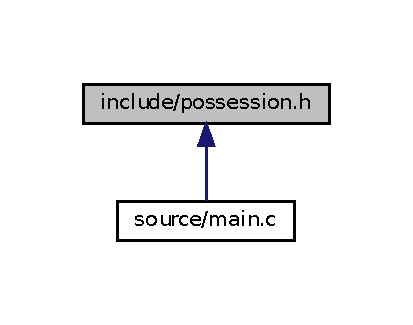
\includegraphics[width=198pt]{possession_8h__dep__incl}
\end{center}
\end{figure}
\subsection*{Functions}
\begin{DoxyCompactItemize}
\item 
void \mbox{\hyperlink{possession_8h_ab34276d7ffa28da384e2668dcc08b6cd}{possession\+\_\+run}} (M\+P\+I\+\_\+\+Datatype mpi\+\_\+possession\+\_\+envelope, M\+P\+I\+\_\+\+Datatype mpi\+\_\+output\+\_\+envelope, unsigned long K)
\begin{DoxyCompactList}\small\item\em Starts the possession process, which computes ball possessions given the player positions. \end{DoxyCompactList}\end{DoxyCompactItemize}


\subsection{Detailed Description}
\mbox{\hyperlink{possession_8c}{possession.\+c}} function declaration. 



\subsection{Function Documentation}
\mbox{\Hypertarget{possession_8h_ab34276d7ffa28da384e2668dcc08b6cd}\label{possession_8h_ab34276d7ffa28da384e2668dcc08b6cd}} 
\index{possession.\+h@{possession.\+h}!possession\+\_\+run@{possession\+\_\+run}}
\index{possession\+\_\+run@{possession\+\_\+run}!possession.\+h@{possession.\+h}}
\subsubsection{\texorpdfstring{possession\+\_\+run()}{possession\_run()}}
{\footnotesize\ttfamily void possession\+\_\+run (\begin{DoxyParamCaption}\item[{M\+P\+I\+\_\+\+Datatype}]{mpi\+\_\+possession\+\_\+envelope,  }\item[{M\+P\+I\+\_\+\+Datatype}]{mpi\+\_\+output\+\_\+envelope,  }\item[{unsigned long}]{K }\end{DoxyParamCaption})}



Starts the possession process, which computes ball possessions given the player positions. 

It keeps waiting for P\+O\+S\+I\+T\+I\+O\+N\+S\+\_\+\+M\+E\+S\+S\+A\+GE containing players or ball position updates, until receiving the E\+N\+D\+O\+F\+G\+A\+M\+E\+\_\+\+M\+E\+S\+S\+A\+GE or an unknown tag message causing the process to abort.

After receiving a P\+O\+S\+I\+T\+I\+O\+N\+S\+\_\+\+M\+E\+S\+S\+A\+GE, it recomputes ball possession\+: a player is considered in possession of the ball when
\begin{DoxyItemize}
\item He is the player closest to the ball
\item He is not farther than K millimeters from the ball. Then it sends an to the \mbox{\hyperlink{output_8c}{output.\+c}} process, which will use it to compute and print the game statistics.
\end{DoxyItemize}

After receiving a E\+N\+D\+O\+F\+G\+A\+M\+E\+\_\+\+M\+E\+S\+S\+A\+GE, it waits for the sending queue to clear out and abort.


\begin{DoxyParams}{Parameters}
{\em mpi\+\_\+possession\+\_\+envelope} & mpi\+\_\+datatype of received message from \mbox{\hyperlink{parser_8h_a6b4f69b75cefd464a448d7dbf87576fa}{parser\+\_\+run}} process, with tag P\+O\+S\+I\+T\+I\+O\+N\+S\+\_\+\+M\+E\+S\+S\+A\+GE or E\+N\+D\+O\+F\+G\+A\+M\+E\+\_\+\+M\+E\+S\+S\+A\+GE. \\
\hline
{\em mpi\+\_\+output\+\_\+envelope} & mpi\+\_\+datatype of sent messages to output process. \\
\hline
{\em K} & Maximum distance between ball and player\+: if distance between each player and the ball is greater than k then no one has ball possession. K is in millimeters and ranges from 1000 to 5000. \\
\hline
\end{DoxyParams}


Definition at line 57 of file possession.\+c.


\hypertarget{main_8c}{}\section{source/main.c File Reference}
\label{main_8c}\index{source/main.\+c@{source/main.\+c}}


This file contains the main function which starts the program.  


{\ttfamily \#include $<$stdio.\+h$>$}\newline
{\ttfamily \#include $<$stdlib.\+h$>$}\newline
{\ttfamily \#include $<$unistd.\+h$>$}\newline
{\ttfamily \#include $<$stddef.\+h$>$}\newline
{\ttfamily \#include \char`\"{}common.\+h\char`\"{}}\newline
{\ttfamily \#include \char`\"{}parser.\+h\char`\"{}}\newline
{\ttfamily \#include \char`\"{}possession.\+h\char`\"{}}\newline
{\ttfamily \#include \char`\"{}output.\+h\char`\"{}}\newline
Include dependency graph for main.\+c\+:\nopagebreak
\begin{figure}[H]
\begin{center}
\leavevmode
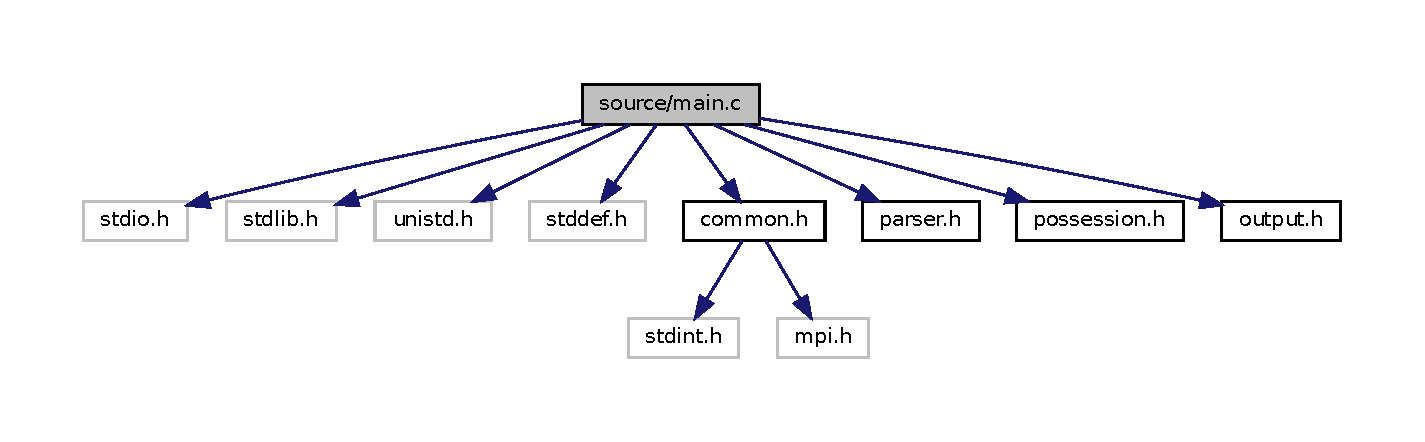
\includegraphics[width=350pt]{main_8c__incl}
\end{center}
\end{figure}
\subsection*{Functions}
\begin{DoxyCompactItemize}
\item 
\mbox{\Hypertarget{main_8c_a0ddf1224851353fc92bfbff6f499fa97}\label{main_8c_a0ddf1224851353fc92bfbff6f499fa97}} 
int {\bfseries main} (int argc, char $\ast$argv\mbox{[}$\,$\mbox{]})
\end{DoxyCompactItemize}


\subsection{Detailed Description}
This file contains the main function which starts the program. 

After setting the user-\/given interval (T in seconds) and possession distance (K in meters), it initializes the M\+PI execution environment and the M\+PI datatypes. Given the number of runnable process N, it starts the parser and output processes and N-\/2 possession process. After all children process have finished it terminates the M\+PI execution environment and returns. 
\hypertarget{output_8c}{}\section{source/output.c File Reference}
\label{output_8c}\index{source/output.\+c@{source/output.\+c}}


This file defines a process, initialize by \mbox{\hyperlink{main_8c}{main.\+c}}, whose job is to compute and output the statistic of the game for each team and player.  


{\ttfamily \#include $<$stdio.\+h$>$}\newline
{\ttfamily \#include \char`\"{}common.\+h\char`\"{}}\newline
Include dependency graph for output.\+c\+:\nopagebreak
\begin{figure}[H]
\begin{center}
\leavevmode
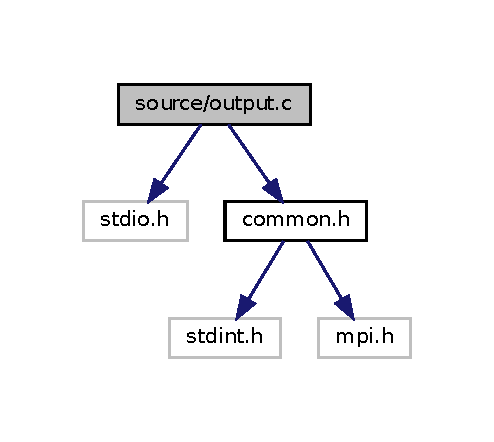
\includegraphics[width=237pt]{output_8c__incl}
\end{center}
\end{figure}
\subsection*{Functions}
\begin{DoxyCompactItemize}
\item 
void \mbox{\hyperlink{output_8c_ab1b9452bfe2baf53184a88e3c2f7ca8d}{print\+\_\+interval}} (int interval, \mbox{\hyperlink{common_8h_aa141e5aeed9e5c126c44e1e0ca46a917}{picoseconds}} T)
\begin{DoxyCompactList}\small\item\em Prints the interval header with the current game time. \end{DoxyCompactList}\item 
void \mbox{\hyperlink{output_8c_a626f2ff222e91340bf8f672a198601a9}{print\+\_\+statistics}} (const unsigned int $\ast$interval\+\_\+possession, const unsigned int $\ast$total\+\_\+possession, int interval, \mbox{\hyperlink{common_8h_aa141e5aeed9e5c126c44e1e0ca46a917}{picoseconds}} T)
\begin{DoxyCompactList}\small\item\em Prints for every team and every member last interval statistic, followed by current cumulative statistics. \end{DoxyCompactList}\item 
void \mbox{\hyperlink{output_8c_ac43f98545e1da1dbf0dff2d81ec06aef}{output\+\_\+run}} (M\+P\+I\+\_\+\+Datatype mpi\+\_\+output\+\_\+envelope, \mbox{\hyperlink{common_8h_aa141e5aeed9e5c126c44e1e0ca46a917}{picoseconds}} T)
\begin{DoxyCompactList}\small\item\em Starts the output process. \end{DoxyCompactList}\end{DoxyCompactItemize}
\subsection*{Variables}
\begin{DoxyCompactItemize}
\item 
const char $\ast$ \mbox{\hyperlink{output_8c_a4ad762fe82ecb0c253b1521711fb60d7}{player\+\_\+names}} \mbox{[}$\,$\mbox{]}
\begin{DoxyCompactList}\small\item\em Names corresponding to each player id. \end{DoxyCompactList}\end{DoxyCompactItemize}
\textbf{ }\par
\begin{DoxyCompactItemize}
\item 
\mbox{\Hypertarget{output_8c_a301a8ad7a8b07c6201a97ffbdb871896}\label{output_8c_a301a8ad7a8b07c6201a97ffbdb871896}} 
const \mbox{\hyperlink{common_8h_aa141e5aeed9e5c126c44e1e0ca46a917}{picoseconds}} \mbox{\hyperlink{output_8c_a301a8ad7a8b07c6201a97ffbdb871896}{F\+I\+R\+S\+T\+\_\+\+H\+A\+L\+F\+\_\+\+D\+U\+R\+A\+T\+I\+ON}} = \mbox{\hyperlink{common_8h_a00be8e922ee8c3e14442893f3dae22e5}{F\+I\+R\+S\+T\+\_\+\+E\+ND}} -\/ \mbox{\hyperlink{common_8h_a08ada8e459d6a78ab832b804fe67f9a1}{G\+A\+M\+E\+\_\+\+S\+T\+A\+RT}}
\begin{DoxyCompactList}\small\item\em Used to print the interval header. \end{DoxyCompactList}\item 
\mbox{\Hypertarget{output_8c_acd8f2c0d984a9baf1cd41fd24e2cd6bd}\label{output_8c_acd8f2c0d984a9baf1cd41fd24e2cd6bd}} 
const \mbox{\hyperlink{common_8h_aa141e5aeed9e5c126c44e1e0ca46a917}{picoseconds}} \mbox{\hyperlink{output_8c_acd8f2c0d984a9baf1cd41fd24e2cd6bd}{S\+E\+C\+O\+N\+D\+\_\+\+H\+A\+L\+F\+\_\+\+D\+U\+R\+A\+T\+I\+ON}} = \mbox{\hyperlink{common_8h_a27f2d53d534caee2fd2b6252ef98abf8}{G\+A\+M\+E\+\_\+\+E\+ND}} -\/ \mbox{\hyperlink{common_8h_ac73ff91e5f59bf1aeff42ba4f522725a}{S\+E\+C\+O\+N\+D\+\_\+\+S\+T\+A\+RT}}
\begin{DoxyCompactList}\small\item\em Used to print the interval header. \end{DoxyCompactList}\end{DoxyCompactItemize}



\subsection{Detailed Description}
This file defines a process, initialize by \mbox{\hyperlink{main_8c}{main.\+c}}, whose job is to compute and output the statistic of the game for each team and player. 



\subsection{Function Documentation}
\mbox{\Hypertarget{output_8c_ac43f98545e1da1dbf0dff2d81ec06aef}\label{output_8c_ac43f98545e1da1dbf0dff2d81ec06aef}} 
\index{output.\+c@{output.\+c}!output\+\_\+run@{output\+\_\+run}}
\index{output\+\_\+run@{output\+\_\+run}!output.\+c@{output.\+c}}
\subsubsection{\texorpdfstring{output\+\_\+run()}{output\_run()}}
{\footnotesize\ttfamily void output\+\_\+run (\begin{DoxyParamCaption}\item[{M\+P\+I\+\_\+\+Datatype}]{mpi\+\_\+output\+\_\+envelope,  }\item[{\mbox{\hyperlink{common_8h_aa141e5aeed9e5c126c44e1e0ca46a917}{picoseconds}}}]{T }\end{DoxyParamCaption})}



Starts the output process. 

It keeps waiting for a P\+R\+I\+N\+T\+\_\+\+M\+E\+S\+S\+A\+GE or a P\+O\+S\+S\+E\+S\+S\+I\+O\+N\+\_\+\+M\+E\+S\+S\+A\+GE, from possession processes, until it receives the E\+N\+D\+\_\+\+O\+F\+\_\+\+G\+A\+ME message. After receiving a P\+O\+S\+S\+E\+S\+S\+I\+O\+N\+\_\+\+M\+E\+S\+S\+A\+GE, statistics are updated; after receiving a P\+R\+I\+N\+T\+\_\+\+M\+E\+S\+S\+A\+GE, interval and cumulative statistics are printed, and interval ones are reset; after receiving the E\+N\+D\+\_\+\+O\+F\+\_\+\+G\+A\+ME message, the process exits, after waiting for any pending request. If the received message is of any other type, the process abort.


\begin{DoxyParams}{Parameters}
{\em mpi\+\_\+output\+\_\+envelope} & M\+PI datatype of the received messages. \\
\hline
{\em T} & Length of time between outputs \\
\hline
\end{DoxyParams}


Definition at line 203 of file output.\+c.

\mbox{\Hypertarget{output_8c_ab1b9452bfe2baf53184a88e3c2f7ca8d}\label{output_8c_ab1b9452bfe2baf53184a88e3c2f7ca8d}} 
\index{output.\+c@{output.\+c}!print\+\_\+interval@{print\+\_\+interval}}
\index{print\+\_\+interval@{print\+\_\+interval}!output.\+c@{output.\+c}}
\subsubsection{\texorpdfstring{print\+\_\+interval()}{print\_interval()}}
{\footnotesize\ttfamily void print\+\_\+interval (\begin{DoxyParamCaption}\item[{int}]{interval,  }\item[{\mbox{\hyperlink{common_8h_aa141e5aeed9e5c126c44e1e0ca46a917}{picoseconds}}}]{T }\end{DoxyParamCaption})}



Prints the interval header with the current game time. 


\begin{DoxyParams}{Parameters}
{\em interval} & Current interval id. \\
\hline
{\em T} & Interval length (in picoseconds). \\
\hline
\end{DoxyParams}


Definition at line 43 of file output.\+c.

\mbox{\Hypertarget{output_8c_a626f2ff222e91340bf8f672a198601a9}\label{output_8c_a626f2ff222e91340bf8f672a198601a9}} 
\index{output.\+c@{output.\+c}!print\+\_\+statistics@{print\+\_\+statistics}}
\index{print\+\_\+statistics@{print\+\_\+statistics}!output.\+c@{output.\+c}}
\subsubsection{\texorpdfstring{print\+\_\+statistics()}{print\_statistics()}}
{\footnotesize\ttfamily void print\+\_\+statistics (\begin{DoxyParamCaption}\item[{const unsigned int $\ast$}]{interval\+\_\+possession,  }\item[{const unsigned int $\ast$}]{total\+\_\+possession,  }\item[{int}]{interval,  }\item[{\mbox{\hyperlink{common_8h_aa141e5aeed9e5c126c44e1e0ca46a917}{picoseconds}}}]{T }\end{DoxyParamCaption})}



Prints for every team and every member last interval statistic, followed by current cumulative statistics. 


\begin{DoxyParams}{Parameters}
{\em interval\+\_\+possession} & Array with last interval statistics for every player (each identified by a constant position in the array). \\
\hline
{\em total\+\_\+possession} & Array with cumulative statistics for every player (each identified by a constant position in the array). \\
\hline
{\em interval} & Incrementing value used to identify each interval of time. \\
\hline
\end{DoxyParams}


Definition at line 74 of file output.\+c.



\subsection{Variable Documentation}
\mbox{\Hypertarget{output_8c_a4ad762fe82ecb0c253b1521711fb60d7}\label{output_8c_a4ad762fe82ecb0c253b1521711fb60d7}} 
\index{output.\+c@{output.\+c}!player\+\_\+names@{player\+\_\+names}}
\index{player\+\_\+names@{player\+\_\+names}!output.\+c@{output.\+c}}
\subsubsection{\texorpdfstring{player\+\_\+names}{player\_names}}
{\footnotesize\ttfamily const char$\ast$ player\+\_\+names\mbox{[}$\,$\mbox{]}}

{\bfseries Initial value\+:}
\begin{DoxyCode}
= \{\textcolor{stringliteral}{"None"},
                              \textcolor{stringliteral}{"Nick Gertje"},
                              \textcolor{stringliteral}{"Dennis Dotterweich"},
                              \textcolor{stringliteral}{"Niklas Waelzlein"},
                              \textcolor{stringliteral}{"Wili Sommer"},
                              \textcolor{stringliteral}{"Philipp Harlass"},
                              \textcolor{stringliteral}{"Roman Hartleb"},
                              \textcolor{stringliteral}{"Erik Engelhardt"},
                              \textcolor{stringliteral}{"Sandro Schneider"},
                              \textcolor{stringliteral}{"Leon Krapf"},
                              \textcolor{stringliteral}{"Kevin Baer"},
                              \textcolor{stringliteral}{"Luca Ziegler"},
                              \textcolor{stringliteral}{"Ben Mueller"},
                              \textcolor{stringliteral}{"Vale Reitstetter"},
                              \textcolor{stringliteral}{"Christopher Lee"},
                              \textcolor{stringliteral}{"Leon Heinze"},
                              \textcolor{stringliteral}{"Leo Langhans"}\}
\end{DoxyCode}


Names corresponding to each player id. 



Definition at line 13 of file output.\+c.


\hypertarget{parser_8c}{}\section{source/parser.c File Reference}
\label{parser_8c}\index{source/parser.\+c@{source/parser.\+c}}


This file defines a process, initialized by \mbox{\hyperlink{main_8c}{main.\+c}}, whose job is to read game data.  


{\ttfamily \#include $<$stdio.\+h$>$}\newline
{\ttfamily \#include $<$stdlib.\+h$>$}\newline
{\ttfamily \#include $<$stdbool.\+h$>$}\newline
{\ttfamily \#include \char`\"{}common.\+h\char`\"{}}\newline
Include dependency graph for parser.\+c\+:\nopagebreak
\begin{figure}[H]
\begin{center}
\leavevmode
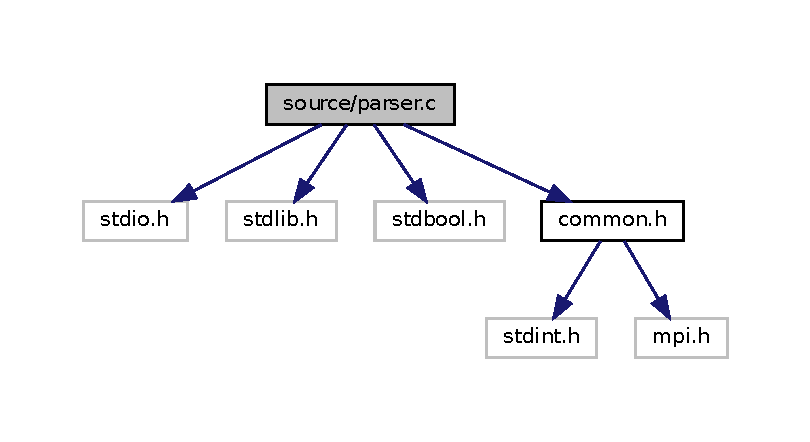
\includegraphics[width=350pt]{parser_8c__incl}
\end{center}
\end{figure}
\subsection*{Functions}
\begin{DoxyCompactItemize}
\item 
\mbox{\hyperlink{common_8h_a089f166159fb19f10d81c65c1d8793a2}{sensor\+\_\+type\+\_\+t}} \mbox{\hyperlink{parser_8c_abeb296b7da9357c17c7d4698c4a313a7}{get\+\_\+sensor\+\_\+type}} (\mbox{\hyperlink{common_8h_af10e2dceeefdc0af7b5bab152a6380d2}{sid\+\_\+t}} sid)
\begin{DoxyCompactList}\small\item\em Given the sensor id it return the sensor type. \end{DoxyCompactList}\item 
\mbox{\hyperlink{common_8h_a7236ef194cc4c2220b9f7dc5e4777f22}{player\+\_\+t}} \mbox{\hyperlink{parser_8c_a01fe702277fddbbefb5be63b3c683b0a}{get\+\_\+sensor\+\_\+player}} (\mbox{\hyperlink{common_8h_af10e2dceeefdc0af7b5bab152a6380d2}{sid\+\_\+t}} sid)
\begin{DoxyCompactList}\small\item\em Given the sensor id of a player, return the player. \end{DoxyCompactList}\item 
bool \mbox{\hyperlink{parser_8c_ab4059b6d956e5231015b6c3a8dadf40e}{ball\+\_\+is\+\_\+in\+\_\+play}} (\mbox{\hyperlink{structposition}{position}} p)
\begin{DoxyCompactList}\small\item\em Returns T\+R\+UE if the given position is within the field. \end{DoxyCompactList}\item 
void \mbox{\hyperlink{parser_8c_a1dd14eda4036f3237ebbcf382cbd50b3}{read\+Event}} (F\+I\+LE $\ast$file, \mbox{\hyperlink{structevent}{event}} $\ast$new)
\begin{DoxyCompactList}\small\item\em Reads an event from the file and returns it as a new object. \end{DoxyCompactList}\item 
int \mbox{\hyperlink{parser_8c_a4da18fef04f82d61a63e0bd181ca0984}{read\+Interruption\+Event}} (F\+I\+LE $\ast$$\ast$file, struct \mbox{\hyperlink{structinterruption__event}{interruption\+\_\+event}} $\ast$new, \mbox{\hyperlink{common_8h_aa141e5aeed9e5c126c44e1e0ca46a917}{picoseconds}} start)
\begin{DoxyCompactList}\small\item\em Reads a new interruption event from file and store read data in the new \mbox{\hyperlink{structinterruption__event}{interruption\+\_\+event}}. \end{DoxyCompactList}\item 
void \mbox{\hyperlink{parser_8c_a6b4f69b75cefd464a448d7dbf87576fa}{parser\+\_\+run}} (M\+P\+I\+\_\+\+Datatype mpi\+\_\+position\+\_\+for\+\_\+possession\+\_\+type, M\+P\+I\+\_\+\+Datatype mpi\+\_\+output\+\_\+envelope, int possession\+\_\+processes, \mbox{\hyperlink{common_8h_aa141e5aeed9e5c126c44e1e0ca46a917}{picoseconds}} T, char $\ast$fullgame\+\_\+path, char $\ast$interr\+\_\+path\+\_\+one, char $\ast$interr\+\_\+path\+\_\+two)
\begin{DoxyCompactList}\small\item\em Starts the parser, which receives events from all sensors and communicates with the output and possession processes. \end{DoxyCompactList}\end{DoxyCompactItemize}
\subsection*{Variables}
\begin{DoxyCompactItemize}
\item 
const \mbox{\hyperlink{common_8h_a089f166159fb19f10d81c65c1d8793a2}{sensor\+\_\+type\+\_\+t}} \mbox{\hyperlink{parser_8c_a2bce9557be0b36b68488cb171112bbb3}{sensor\+\_\+type\+\_\+list}} \mbox{[}$\,$\mbox{]}
\item 
const \mbox{\hyperlink{common_8h_a7236ef194cc4c2220b9f7dc5e4777f22}{player\+\_\+t}} \mbox{\hyperlink{parser_8c_ad89c030cddfeca6e74b95a93b96505ab}{sensor\+\_\+player\+\_\+list}} \mbox{[}$\,$\mbox{]}
\end{DoxyCompactItemize}


\subsection{Detailed Description}
This file defines a process, initialized by \mbox{\hyperlink{main_8c}{main.\+c}}, whose job is to read game data. 



\subsection{Function Documentation}
\mbox{\Hypertarget{parser_8c_ab4059b6d956e5231015b6c3a8dadf40e}\label{parser_8c_ab4059b6d956e5231015b6c3a8dadf40e}} 
\index{parser.\+c@{parser.\+c}!ball\+\_\+is\+\_\+in\+\_\+play@{ball\+\_\+is\+\_\+in\+\_\+play}}
\index{ball\+\_\+is\+\_\+in\+\_\+play@{ball\+\_\+is\+\_\+in\+\_\+play}!parser.\+c@{parser.\+c}}
\subsubsection{\texorpdfstring{ball\+\_\+is\+\_\+in\+\_\+play()}{ball\_is\_in\_play()}}
{\footnotesize\ttfamily bool ball\+\_\+is\+\_\+in\+\_\+play (\begin{DoxyParamCaption}\item[{\mbox{\hyperlink{structposition}{position}}}]{p }\end{DoxyParamCaption})}



Returns T\+R\+UE if the given position is within the field. 


\begin{DoxyParams}{Parameters}
{\em p} & Ball position. \\
\hline
\end{DoxyParams}
\begin{DoxyReturn}{Returns}
a bool. 
\end{DoxyReturn}


Definition at line 88 of file parser.\+c.

\mbox{\Hypertarget{parser_8c_a01fe702277fddbbefb5be63b3c683b0a}\label{parser_8c_a01fe702277fddbbefb5be63b3c683b0a}} 
\index{parser.\+c@{parser.\+c}!get\+\_\+sensor\+\_\+player@{get\+\_\+sensor\+\_\+player}}
\index{get\+\_\+sensor\+\_\+player@{get\+\_\+sensor\+\_\+player}!parser.\+c@{parser.\+c}}
\subsubsection{\texorpdfstring{get\+\_\+sensor\+\_\+player()}{get\_sensor\_player()}}
{\footnotesize\ttfamily \mbox{\hyperlink{common_8h_a7236ef194cc4c2220b9f7dc5e4777f22}{player\+\_\+t}} get\+\_\+sensor\+\_\+player (\begin{DoxyParamCaption}\item[{\mbox{\hyperlink{common_8h_af10e2dceeefdc0af7b5bab152a6380d2}{sid\+\_\+t}}}]{sid }\end{DoxyParamCaption})}



Given the sensor id of a player, return the player. 


\begin{DoxyParams}{Parameters}
{\em sid} & Sensor id. \\
\hline
\end{DoxyParams}
\begin{DoxyReturn}{Returns}
Id of the player as player\+\_\+t. 
\end{DoxyReturn}


Definition at line 70 of file parser.\+c.

\mbox{\Hypertarget{parser_8c_abeb296b7da9357c17c7d4698c4a313a7}\label{parser_8c_abeb296b7da9357c17c7d4698c4a313a7}} 
\index{parser.\+c@{parser.\+c}!get\+\_\+sensor\+\_\+type@{get\+\_\+sensor\+\_\+type}}
\index{get\+\_\+sensor\+\_\+type@{get\+\_\+sensor\+\_\+type}!parser.\+c@{parser.\+c}}
\subsubsection{\texorpdfstring{get\+\_\+sensor\+\_\+type()}{get\_sensor\_type()}}
{\footnotesize\ttfamily \mbox{\hyperlink{common_8h_a089f166159fb19f10d81c65c1d8793a2}{sensor\+\_\+type\+\_\+t}} get\+\_\+sensor\+\_\+type (\begin{DoxyParamCaption}\item[{\mbox{\hyperlink{common_8h_af10e2dceeefdc0af7b5bab152a6380d2}{sid\+\_\+t}}}]{sid }\end{DoxyParamCaption})}



Given the sensor id it return the sensor type. 


\begin{DoxyParams}{Parameters}
{\em sid} & Sensor id. \\
\hline
\end{DoxyParams}
\begin{DoxyReturn}{Returns}
Sensor type; N\+O\+NE, B\+A\+LL, P\+L\+A\+Y\+ER or R\+E\+F\+E\+R\+EE. 
\end{DoxyReturn}


Definition at line 52 of file parser.\+c.

\mbox{\Hypertarget{parser_8c_a6b4f69b75cefd464a448d7dbf87576fa}\label{parser_8c_a6b4f69b75cefd464a448d7dbf87576fa}} 
\index{parser.\+c@{parser.\+c}!parser\+\_\+run@{parser\+\_\+run}}
\index{parser\+\_\+run@{parser\+\_\+run}!parser.\+c@{parser.\+c}}
\subsubsection{\texorpdfstring{parser\+\_\+run()}{parser\_run()}}
{\footnotesize\ttfamily void parser\+\_\+run (\begin{DoxyParamCaption}\item[{M\+P\+I\+\_\+\+Datatype}]{mpi\+\_\+position\+\_\+for\+\_\+possession\+\_\+type,  }\item[{M\+P\+I\+\_\+\+Datatype}]{mpi\+\_\+output\+\_\+envelope,  }\item[{int}]{possession\+\_\+processes,  }\item[{\mbox{\hyperlink{common_8h_aa141e5aeed9e5c126c44e1e0ca46a917}{picoseconds}}}]{T,  }\item[{char $\ast$}]{fullgame\+\_\+path,  }\item[{char $\ast$}]{interr\+\_\+path\+\_\+one,  }\item[{char $\ast$}]{interr\+\_\+path\+\_\+two }\end{DoxyParamCaption})}



Starts the parser, which receives events from all sensors and communicates with the output and possession processes. 

Start, end and interruptions of the game are highlighted in the data received by the process.


\begin{DoxyParams}{Parameters}
{\em mpi\+\_\+position\+\_\+for\+\_\+possession\+\_\+type} & M\+PI datatype used to send messages to the possession process \\
\hline
{\em mpi\+\_\+output\+\_\+envelope} & M\+PI datatype used to send messages to the output process \\
\hline
{\em possession\+\_\+processes} & Number of possession processes that are running, used to know buffer sizes \\
\hline
{\em T} & Length of time between outputs \\
\hline
{\em fullgame\+\_\+path} & Path for the position events file \\
\hline
{\em interr\+\_\+path\+\_\+one} & Path for the first game interruptions file \\
\hline
{\em interr\+\_\+path\+\_\+two} & Path for the second game interruptions file \\
\hline
\end{DoxyParams}


Definition at line 147 of file parser.\+c.

\mbox{\Hypertarget{parser_8c_a1dd14eda4036f3237ebbcf382cbd50b3}\label{parser_8c_a1dd14eda4036f3237ebbcf382cbd50b3}} 
\index{parser.\+c@{parser.\+c}!read\+Event@{read\+Event}}
\index{read\+Event@{read\+Event}!parser.\+c@{parser.\+c}}
\subsubsection{\texorpdfstring{read\+Event()}{readEvent()}}
{\footnotesize\ttfamily void read\+Event (\begin{DoxyParamCaption}\item[{F\+I\+LE $\ast$}]{file,  }\item[{\mbox{\hyperlink{structevent}{event}} $\ast$}]{new }\end{DoxyParamCaption})}



Reads an event from the file and returns it as a new object. 


\begin{DoxyParams}{Parameters}
{\em file} & An open file pointer to read from \\
\hline
{\em new} & A pointer to a free event buffer to write the new event to \\
\hline
\end{DoxyParams}


Definition at line 97 of file parser.\+c.

\mbox{\Hypertarget{parser_8c_a4da18fef04f82d61a63e0bd181ca0984}\label{parser_8c_a4da18fef04f82d61a63e0bd181ca0984}} 
\index{parser.\+c@{parser.\+c}!read\+Interruption\+Event@{read\+Interruption\+Event}}
\index{read\+Interruption\+Event@{read\+Interruption\+Event}!parser.\+c@{parser.\+c}}
\subsubsection{\texorpdfstring{read\+Interruption\+Event()}{readInterruptionEvent()}}
{\footnotesize\ttfamily int read\+Interruption\+Event (\begin{DoxyParamCaption}\item[{F\+I\+LE $\ast$$\ast$}]{file,  }\item[{struct \mbox{\hyperlink{structinterruption__event}{interruption\+\_\+event}} $\ast$}]{new,  }\item[{\mbox{\hyperlink{common_8h_aa141e5aeed9e5c126c44e1e0ca46a917}{picoseconds}}}]{start }\end{DoxyParamCaption})}



Reads a new interruption event from file and store read data in the new \mbox{\hyperlink{structinterruption__event}{interruption\+\_\+event}}. 


\begin{DoxyParams}{Parameters}
{\em file} & An open file pointer to read from \\
\hline
{\em new} & A pointer to a free \mbox{\hyperlink{structinterruption__event}{interruption\+\_\+event}} buffer to write the new event to \\
\hline
{\em start} & Start time of the current half of the game. Used as offset for the event time, as the files start from zero \\
\hline
\end{DoxyParams}
\begin{DoxyReturn}{Returns}
0 if everything went ok, non-\/zero if an error occurred 
\end{DoxyReturn}


Definition at line 109 of file parser.\+c.



\subsection{Variable Documentation}
\mbox{\Hypertarget{parser_8c_ad89c030cddfeca6e74b95a93b96505ab}\label{parser_8c_ad89c030cddfeca6e74b95a93b96505ab}} 
\index{parser.\+c@{parser.\+c}!sensor\+\_\+player\+\_\+list@{sensor\+\_\+player\+\_\+list}}
\index{sensor\+\_\+player\+\_\+list@{sensor\+\_\+player\+\_\+list}!parser.\+c@{parser.\+c}}
\subsubsection{\texorpdfstring{sensor\+\_\+player\+\_\+list}{sensor\_player\_list}}
{\footnotesize\ttfamily const \mbox{\hyperlink{common_8h_a7236ef194cc4c2220b9f7dc5e4777f22}{player\+\_\+t}} sensor\+\_\+player\+\_\+list\mbox{[}$\,$\mbox{]}}

{\bfseries Initial value\+:}
\begin{DoxyCode}
= \{0, 0, 0, 0, 0, 0, 0, 0, 0, 0, 0, 0, 0, 1, 1, 0, 2, 0, 0, 4, 0, 0, 0, 6, 6, 0, 0,
                                       0, 8, 0, 0, 0, 0, 0, 0, 0, 0, 0, 13, 0, 14, 0, 0, 0, 16, 0, 0, 2, 0,
       3, 0, 0, 4,
                                       5, 5, 0, 0, 7, 7, 8, 0, 9, 9, 10, 10, 11, 11, 12, 12, 13, 0, 14, 0, 
      15, 15, 16,
                                       0, 0, 0, 0, 0, 0, 0, 0, 0, 0, 0, 0, 3, 0, 0, 0, 0, 0, 0, 0, 0, 1, 1,
       9, 9\}
\end{DoxyCode}
Indexes correspond to sensor ids\+: for each sensor its player id is stored. Index without an associated player id are stored as 0. 

Definition at line 42 of file parser.\+c.

\mbox{\Hypertarget{parser_8c_a2bce9557be0b36b68488cb171112bbb3}\label{parser_8c_a2bce9557be0b36b68488cb171112bbb3}} 
\index{parser.\+c@{parser.\+c}!sensor\+\_\+type\+\_\+list@{sensor\+\_\+type\+\_\+list}}
\index{sensor\+\_\+type\+\_\+list@{sensor\+\_\+type\+\_\+list}!parser.\+c@{parser.\+c}}
\subsubsection{\texorpdfstring{sensor\+\_\+type\+\_\+list}{sensor\_type\_list}}
{\footnotesize\ttfamily const \mbox{\hyperlink{common_8h_a089f166159fb19f10d81c65c1d8793a2}{sensor\+\_\+type\+\_\+t}} sensor\+\_\+type\+\_\+list\mbox{[}$\,$\mbox{]}}

{\bfseries Initial value\+:}
\begin{DoxyCode}
= \{NONE, NONE, NONE, NONE, BALL, NONE, NONE, NONE, BALL, NONE, BALL, NONE, BALL,
                                          PLAYER, PLAYER, NONE, PLAYER, NONE, NONE, PLAYER, NONE, NONE, 
      NONE, PLAYER,
                                          PLAYER, NONE, NONE, NONE, PLAYER, NONE, NONE, NONE, NONE, NONE, 
      NONE, NONE,
                                          NONE, NONE, PLAYER, NONE, PLAYER, NONE, NONE, NONE, PLAYER, NONE,
       NONE,
                                          PLAYER, NONE, PLAYER, NONE, NONE, PLAYER, PLAYER, PLAYER, NONE, 
      NONE, PLAYER,
                                          PLAYER, PLAYER, NONE, PLAYER, PLAYER, PLAYER, PLAYER, PLAYER, 
      PLAYER, PLAYER,
                                          PLAYER, PLAYER, NONE, PLAYER, NONE, PLAYER, PLAYER, PLAYER, NONE,
       NONE, NONE,
                                          NONE, NONE, NONE, NONE, NONE, NONE, NONE, NONE, NONE, PLAYER, 
      NONE, NONE,
                                          NONE, NONE, NONE, NONE, NONE, NONE, PLAYER, PLAYER, PLAYER, 
      PLAYER, NONE,
                                          NONE, NONE, NONE, REFEREE, REFEREE\}
\end{DoxyCode}
Indexes correspond to sensor ids\+: for each sensor its type is stored. Index without an associated sensor id are stored as N\+O\+NE. 

Definition at line 27 of file parser.\+c.


\hypertarget{possession_8c}{}\section{source/possession.c File Reference}
\label{possession_8c}\index{source/possession.\+c@{source/possession.\+c}}


This file defines a process, initialized by \mbox{\hyperlink{main_8c}{main.\+c}}, whose job is to establish which player, and thus team, has the ball, for each game positions update message from the \mbox{\hyperlink{parser_8h_a6b4f69b75cefd464a448d7dbf87576fa}{parser\+\_\+run}} process.  


{\ttfamily \#include $<$stdio.\+h$>$}\newline
{\ttfamily \#include $<$math.\+h$>$}\newline
{\ttfamily \#include \char`\"{}common.\+h\char`\"{}}\newline
Include dependency graph for possession.\+c\+:\nopagebreak
\begin{figure}[H]
\begin{center}
\leavevmode
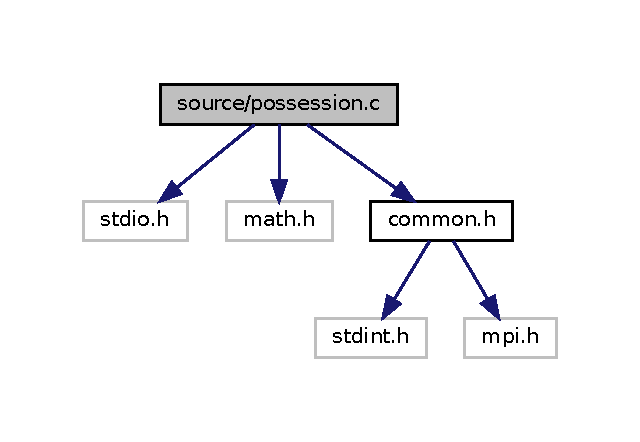
\includegraphics[width=307pt]{possession_8c__incl}
\end{center}
\end{figure}
\subsection*{Functions}
\begin{DoxyCompactItemize}
\item 
double \mbox{\hyperlink{possession_8c_a365f81df4fd3752b09a88c36aa2edfc8}{square\+Distance\+From\+Ball}} (\mbox{\hyperlink{structposition}{position}} player\+\_\+position, \mbox{\hyperlink{structposition}{position}} ball\+\_\+last\+\_\+position)
\begin{DoxyCompactList}\small\item\em This method computes the euclidean distance\textsuperscript{2} between a specific player and the ball. \end{DoxyCompactList}\item 
void \mbox{\hyperlink{possession_8c_ab34276d7ffa28da384e2668dcc08b6cd}{possession\+\_\+run}} (M\+P\+I\+\_\+\+Datatype mpi\+\_\+possession\+\_\+envelope, M\+P\+I\+\_\+\+Datatype mpi\+\_\+output\+\_\+envelope, unsigned long K)
\begin{DoxyCompactList}\small\item\em Starts the possession process, which computes ball possessions given the player positions. \end{DoxyCompactList}\end{DoxyCompactItemize}


\subsection{Detailed Description}
This file defines a process, initialized by \mbox{\hyperlink{main_8c}{main.\+c}}, whose job is to establish which player, and thus team, has the ball, for each game positions update message from the \mbox{\hyperlink{parser_8h_a6b4f69b75cefd464a448d7dbf87576fa}{parser\+\_\+run}} process. 



\subsection{Function Documentation}
\mbox{\Hypertarget{possession_8c_ab34276d7ffa28da384e2668dcc08b6cd}\label{possession_8c_ab34276d7ffa28da384e2668dcc08b6cd}} 
\index{possession.\+c@{possession.\+c}!possession\+\_\+run@{possession\+\_\+run}}
\index{possession\+\_\+run@{possession\+\_\+run}!possession.\+c@{possession.\+c}}
\subsubsection{\texorpdfstring{possession\+\_\+run()}{possession\_run()}}
{\footnotesize\ttfamily void possession\+\_\+run (\begin{DoxyParamCaption}\item[{M\+P\+I\+\_\+\+Datatype}]{mpi\+\_\+possession\+\_\+envelope,  }\item[{M\+P\+I\+\_\+\+Datatype}]{mpi\+\_\+output\+\_\+envelope,  }\item[{unsigned long}]{K }\end{DoxyParamCaption})}



Starts the possession process, which computes ball possessions given the player positions. 

It keeps waiting for P\+O\+S\+I\+T\+I\+O\+N\+S\+\_\+\+M\+E\+S\+S\+A\+GE containing players or ball position updates, until receiving the E\+N\+D\+O\+F\+G\+A\+M\+E\+\_\+\+M\+E\+S\+S\+A\+GE or an unknown tag message causing the process to abort.

After receiving a P\+O\+S\+I\+T\+I\+O\+N\+S\+\_\+\+M\+E\+S\+S\+A\+GE, it recomputes ball possession\+: a player is considered in possession of the ball when
\begin{DoxyItemize}
\item He is the player closest to the ball
\item He is not farther than K millimeters from the ball. Then it sends an to the \mbox{\hyperlink{output_8c}{output.\+c}} process, which will use it to compute and print the game statistics.
\end{DoxyItemize}

After receiving a E\+N\+D\+O\+F\+G\+A\+M\+E\+\_\+\+M\+E\+S\+S\+A\+GE, it waits for the sending queue to clear out and abort.


\begin{DoxyParams}{Parameters}
{\em mpi\+\_\+possession\+\_\+envelope} & mpi\+\_\+datatype of received message from \mbox{\hyperlink{parser_8h_a6b4f69b75cefd464a448d7dbf87576fa}{parser\+\_\+run}} process, with tag P\+O\+S\+I\+T\+I\+O\+N\+S\+\_\+\+M\+E\+S\+S\+A\+GE or E\+N\+D\+O\+F\+G\+A\+M\+E\+\_\+\+M\+E\+S\+S\+A\+GE. \\
\hline
{\em mpi\+\_\+output\+\_\+envelope} & mpi\+\_\+datatype of sent messages to output process. \\
\hline
{\em K} & Maximum distance between ball and player\+: if distance between each player and the ball is greater than k then no one has ball possession. K is in millimeters and ranges from 1000 to 5000. \\
\hline
\end{DoxyParams}


Definition at line 57 of file possession.\+c.

\mbox{\Hypertarget{possession_8c_a365f81df4fd3752b09a88c36aa2edfc8}\label{possession_8c_a365f81df4fd3752b09a88c36aa2edfc8}} 
\index{possession.\+c@{possession.\+c}!square\+Distance\+From\+Ball@{square\+Distance\+From\+Ball}}
\index{square\+Distance\+From\+Ball@{square\+Distance\+From\+Ball}!possession.\+c@{possession.\+c}}
\subsubsection{\texorpdfstring{square\+Distance\+From\+Ball()}{squareDistanceFromBall()}}
{\footnotesize\ttfamily double square\+Distance\+From\+Ball (\begin{DoxyParamCaption}\item[{\mbox{\hyperlink{structposition}{position}}}]{player\+\_\+position,  }\item[{\mbox{\hyperlink{structposition}{position}}}]{ball\+\_\+last\+\_\+position }\end{DoxyParamCaption})}



This method computes the euclidean distance\textsuperscript{2} between a specific player and the ball. 

$distance^2=\sqrt{(x_2-x_1)^2+(y_2-y_1)^2+(z_2-z_1)^2}$


\begin{DoxyParams}{Parameters}
{\em player\+\_\+position} & Position of the player we are interested in. \\
\hline
{\em ball\+\_\+last\+\_\+position} & Ball position. \\
\hline
\end{DoxyParams}
\begin{DoxyReturn}{Returns}
Distance\textsuperscript{2} between player\+\_\+position and ball\+\_\+last\+\_\+position. 
\end{DoxyReturn}


Definition at line 26 of file possession.\+c.


%--- End generated contents ---

% Index
\backmatter
\newpage
\phantomsection
\clearemptydoublepage
\addcontentsline{toc}{chapter}{Index}
\printindex

\end{document}
